\section{1D Solver}
\par Consider the shallow water equations in one dimension,

\begin{equation}
\frac{\partial U}{\partial t} + \frac{\partial F(U)}{\partial x} = 0,
\end{equation}

where $U = [h, hu]^T$ and $F(U) = [hu,\,\, hu^2 + \frac{1}{2} + gh^2]^T$. Define $q(x,t) = u(x,t) h(x,t)$ so we have

\[U = \begin{bmatrix} h, \\ q\end{bmatrix},\,\, F(U) = \begin{bmatrix} q,\\ \frac{q^2}{h} + \frac{1}{2} gh^2 \end{bmatrix}.\]

Let $A$ be a Jacobian of $F(U)$. Thus

\begin{equation}
A = \begin{bmatrix} 0 & 1 \\ -\frac{q^2}{h^2} + gh & \frac{2q}{h}\end{bmatrix}
\end{equation}

with eigenvalues $\lambda = \frac{q}{h} \pm \sqrt{gh}.$ Since $h(x,t) > 0$ and $g$ is a positive constant eigenvalues of the Jacobian are
real and distinct (i.e A has full set of eigenvectors). Hence, the system is hyperbolic. \newline

The Lax-Wendroff method for equation (4) is,
\begin{equation}\label{eqn:4}
U_i^{n+1}=U_i^n-\frac{{\Delta t}}{2}((I-\frac{{\Delta t}}{{\Delta x}}A_{i+1/2}^n)(D_+F_i^n)+((I+\frac{{\Delta
t}}{{\Delta x}}A_{i-1/2}^n)(D_{\_}F_i^n).
\end{equation}
where \(F_i^n=F(U_i^n), A_{i+1/2}\) is the Jacobian matrix of F evaluated at \(U_{i+1/2}\) and \(D_+\) and \(D_-\) are the standard forward
and backward difference operators defined as,
\begin{equation}\label{eqn:5}
D_{\pm }w(x)=\frac{\pm w(x\pm {\Delta x})-\pm w(x))}{{\Delta x}}. 
\end{equation}

Assuming we have \(N_x\) points in the x-direction with \(\Omega =[0\;1]\), and \(1\leq i\leq n\), periodic boundary
conditions can be imposed by \(U_1=U_{N_x}\), reflective boundary conditions at\(x=0\) by \(U_1=-U_2\), and free boundary conditions at \(x=0\) by
\(U_1=U_2\). These equations describe how conditions are imposed on the entire vector U, here we implement reflective boundary
conditions for hu and free boundary conditions for h. The intial conditions are chosen to be interesting, such that
 $h=e^{-(\frac{x-\mu }{\sigma })^2}$ for $u=0$. \newline


\begin{figure}[h!]
    \centering
    \begin{subfigure}[t]{0.48\textwidth}
        \centering
        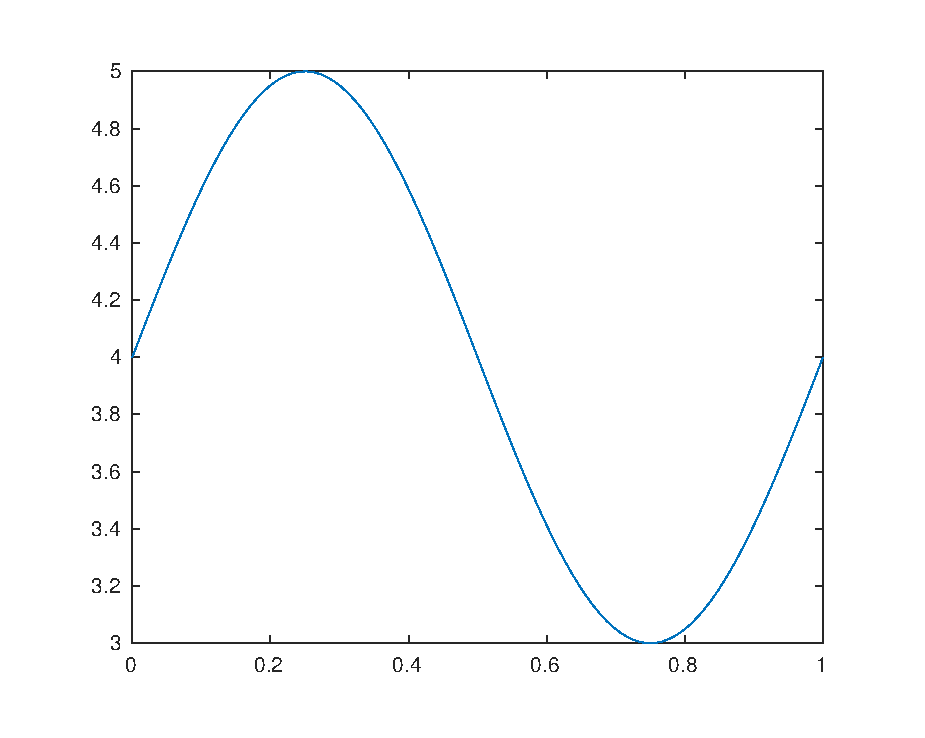
\includegraphics[width=\textwidth]{images/sol_1D_per_0000.eps}
        \caption{$n=0$}
        \label{fig:0}
    \end{subfigure}
    \begin{subfigure}[t]{0.48\textwidth}
        \centering
        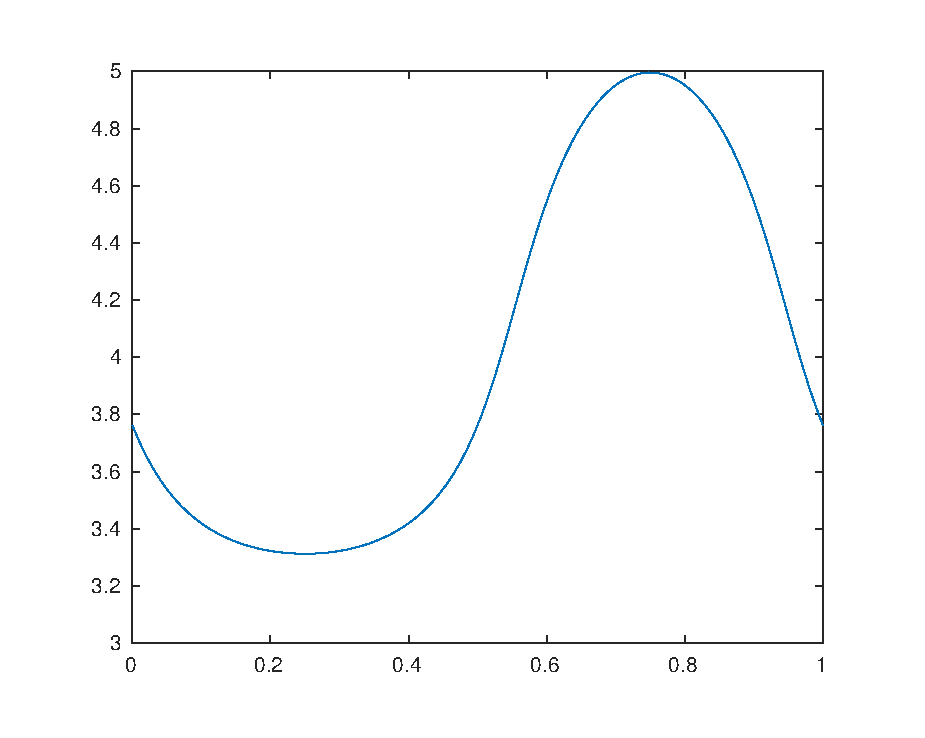
\includegraphics[width=\textwidth]{images/sol_1D_per_0050.eps}
        \caption{$n=50$}
        \label{fig:10}
    \end{subfigure}
    \begin{subfigure}[t]{0.48\textwidth}
        \centering
        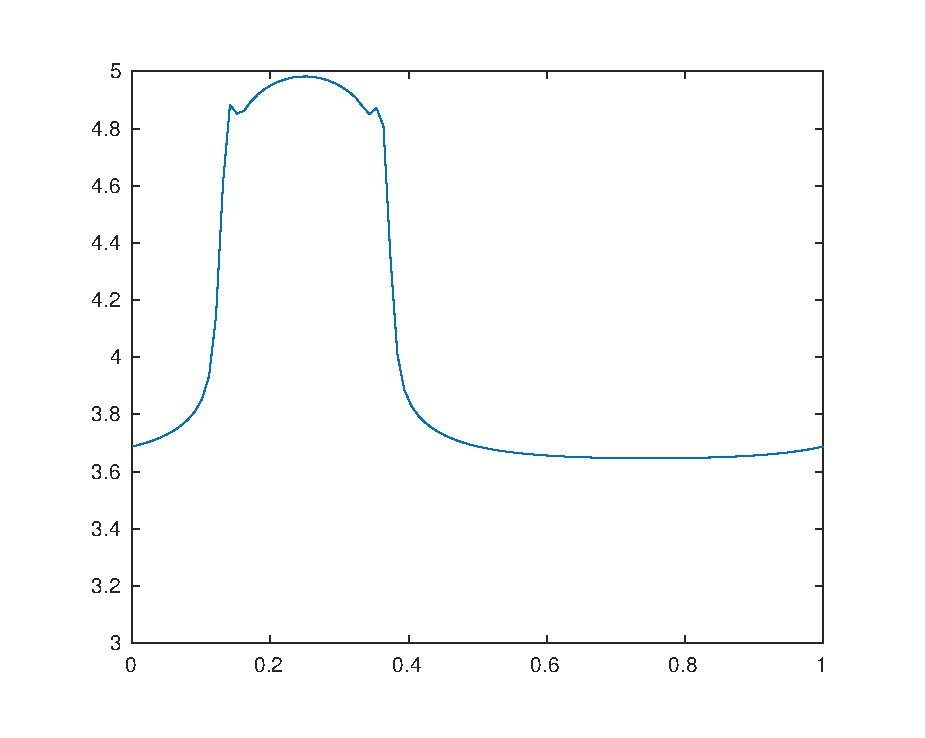
\includegraphics[width=\textwidth]{images/sol_1D_per_0100.eps}
        \caption{$n=100$}
        \label{fig:50}
    \end{subfigure}
    \begin{subfigure}[t]{0.48\textwidth}
        \centering
        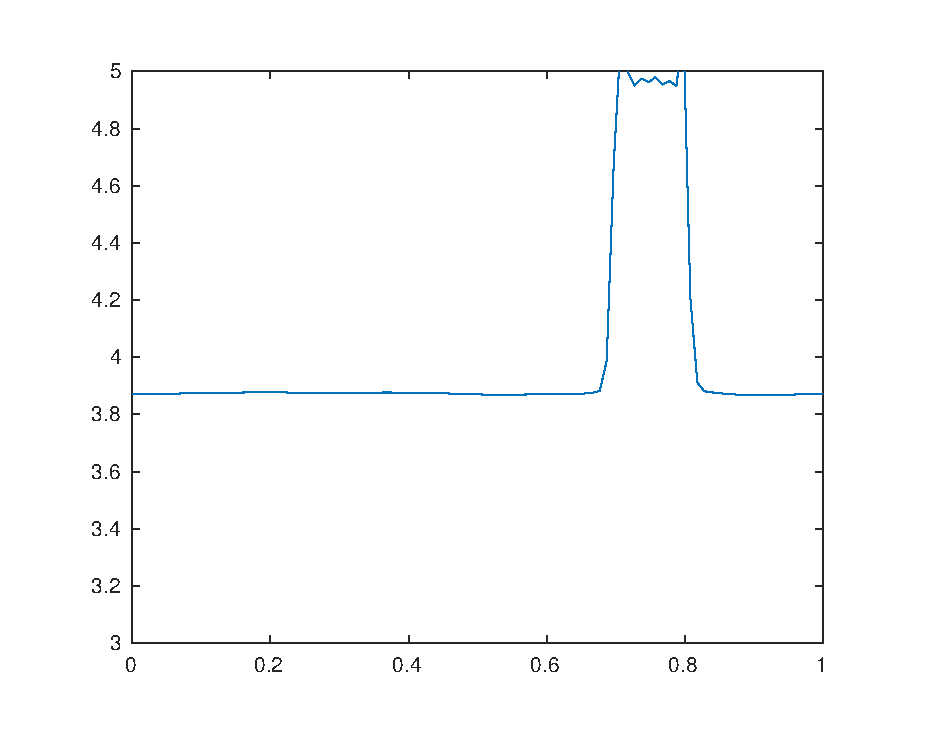
\includegraphics[width=\textwidth]{images/sol_1D_per_0150.eps}
        \caption{$n=150$}
        \label{fig:100}
    \end{subfigure}
    \begin{subfigure}[t]{0.48\textwidth}
        \centering
        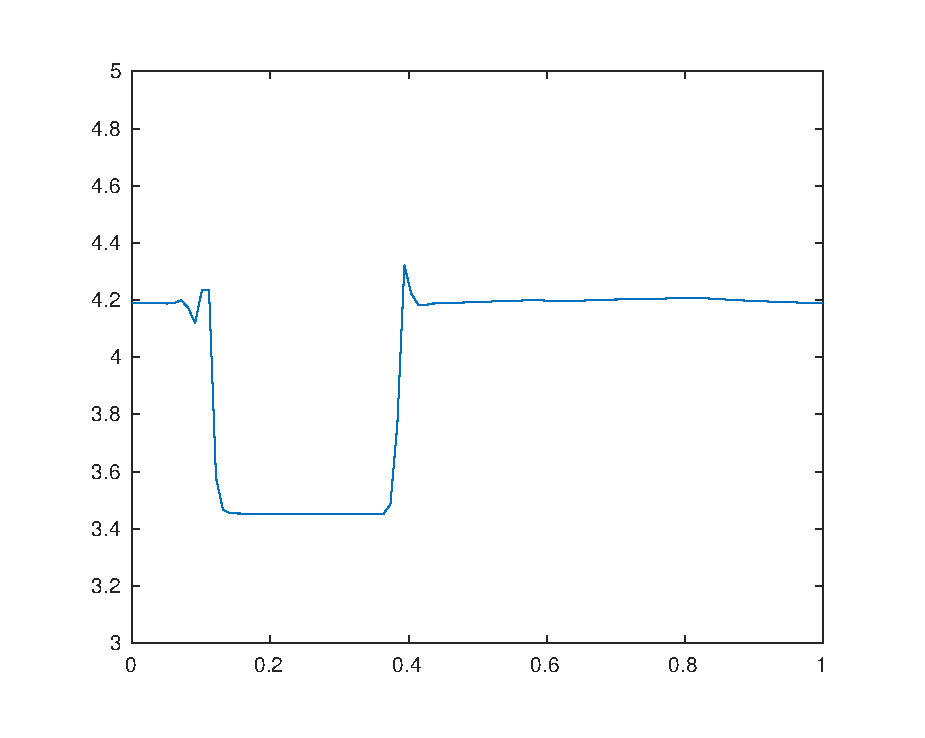
\includegraphics[width=\textwidth]{images/sol_1D_per_0300.eps}
        \caption{$n=300$}
        \label{fig:100}
    \end{subfigure}
    \begin{subfigure}[t]{0.48\textwidth}
        \centering
        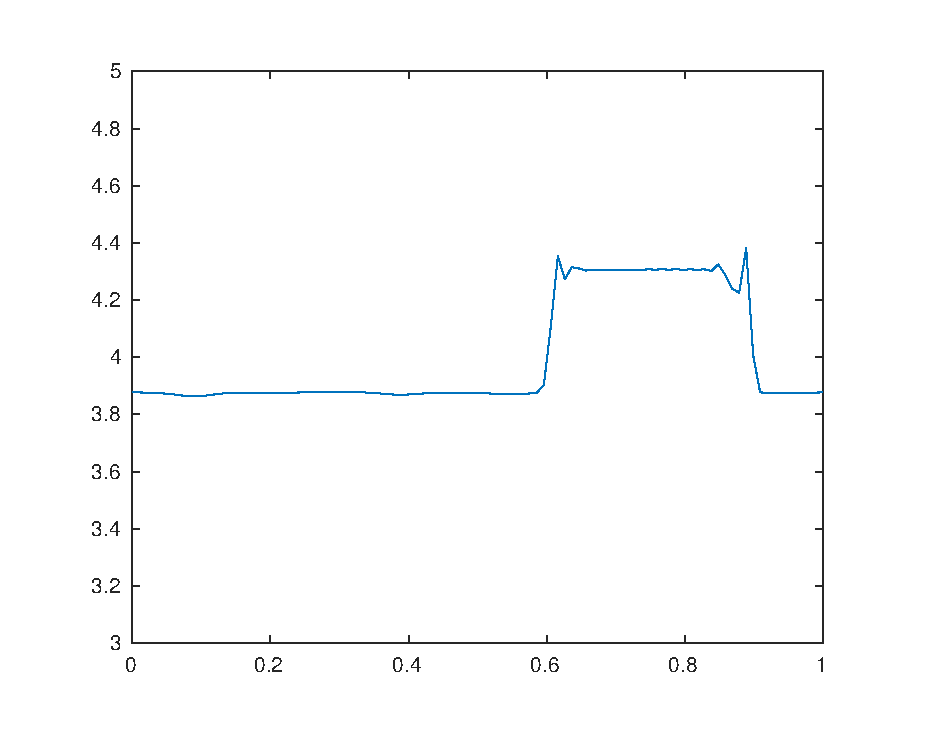
\includegraphics[width=\textwidth]{images/sol_1D_per_0600.eps}
        \caption{$n=600$}
        \label{fig:100}
    \end{subfigure}
     \caption{Periodic boundary conditions for 1D scheme.}
    \label{fig:1DSolutions_per}
\end{figure}

\begin{figure}[h!]
    \centering
    \begin{subfigure}[t]{0.48\textwidth}
        \centering
        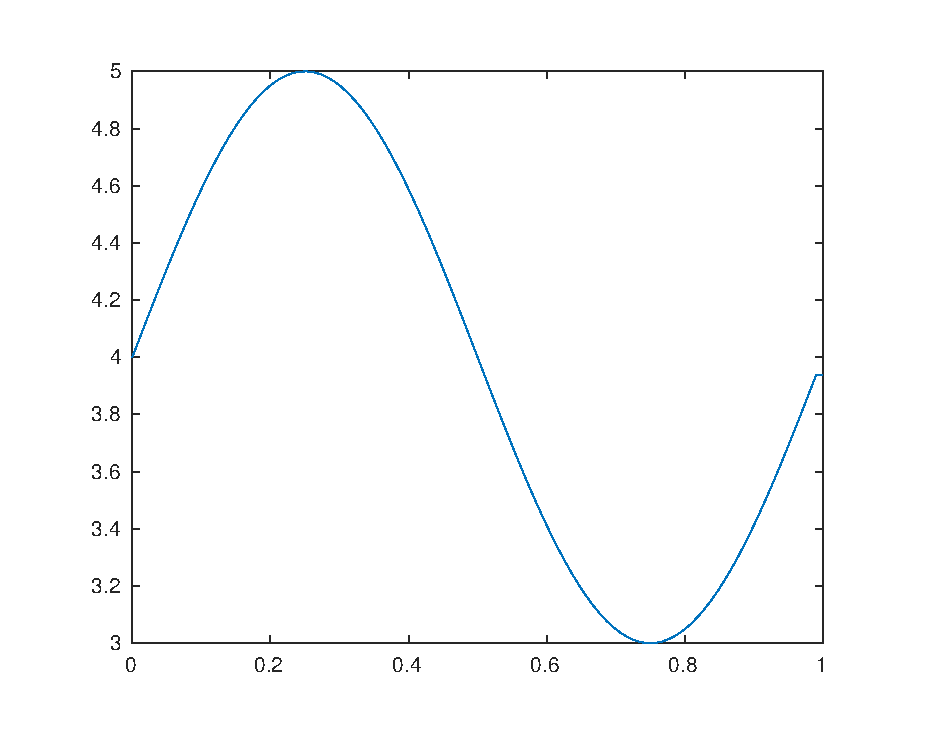
\includegraphics[width=\textwidth]{images/sol_1D_free_0000.eps}
        \caption{$n=0$}
        \label{fig:0}
    \end{subfigure}
    \begin{subfigure}[t]{0.48\textwidth}
        \centering
        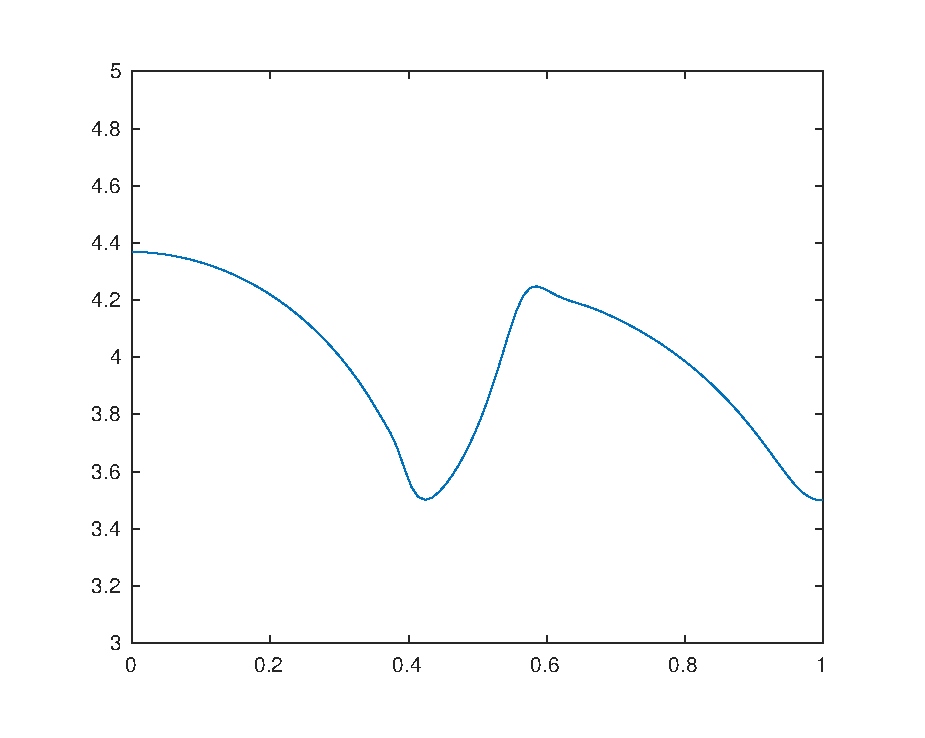
\includegraphics[width=\textwidth]{images/sol_1D_free_0050.eps}
        \caption{$n=50$}
        \label{fig:10}
    \end{subfigure}
    \begin{subfigure}[t]{0.48\textwidth}
        \centering
        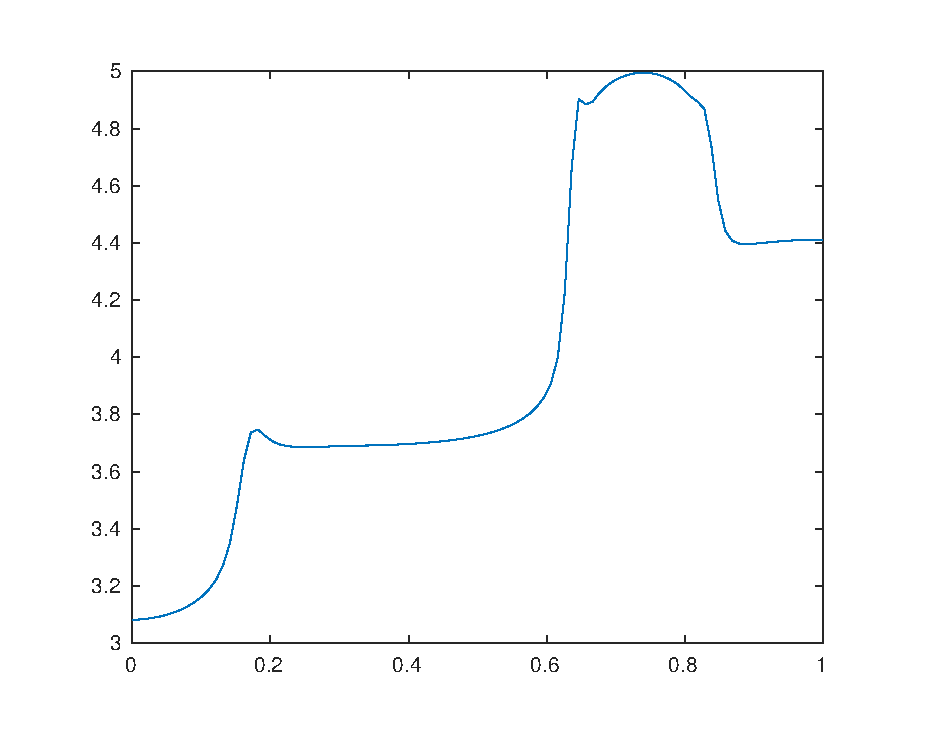
\includegraphics[width=\textwidth]{images/sol_1D_free_0100.eps}
        \caption{$n=100$}
        \label{fig:50}
    \end{subfigure}
    \begin{subfigure}[t]{0.48\textwidth}
        \centering
        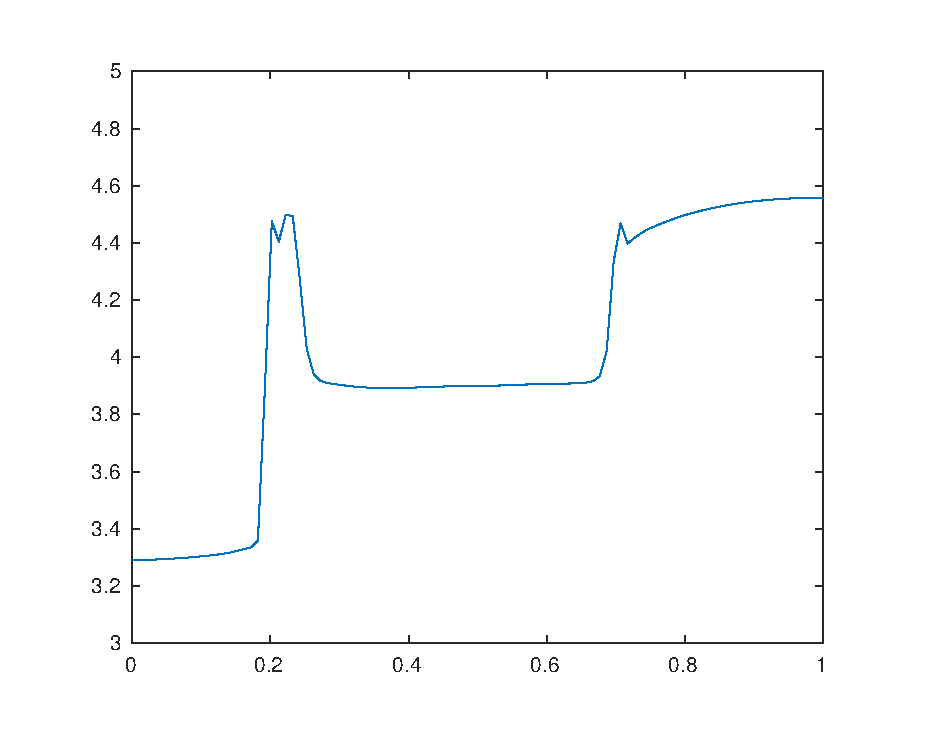
\includegraphics[width=\textwidth]{images/sol_1D_free_0150.eps}
        \caption{$n=150$}
        \label{fig:100}
    \end{subfigure}
    \begin{subfigure}[t]{0.48\textwidth}
        \centering
        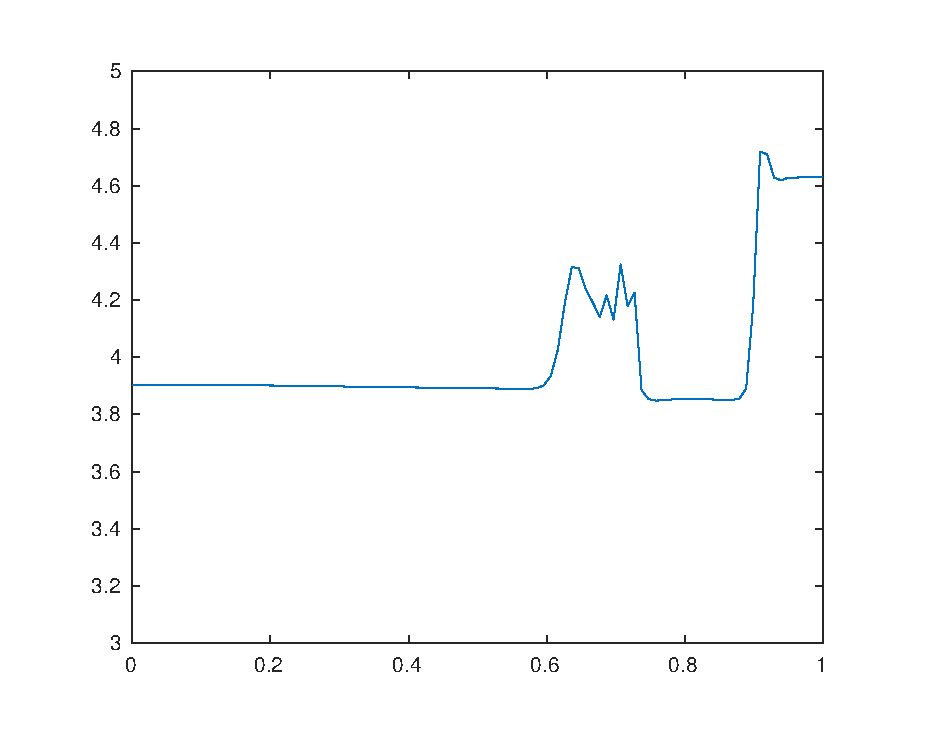
\includegraphics[width=\textwidth]{images/sol_1D_free_0300.eps}
        \caption{$n=300$}
        \label{fig:100}
    \end{subfigure}
    \begin{subfigure}[t]{0.48\textwidth}
        \centering
        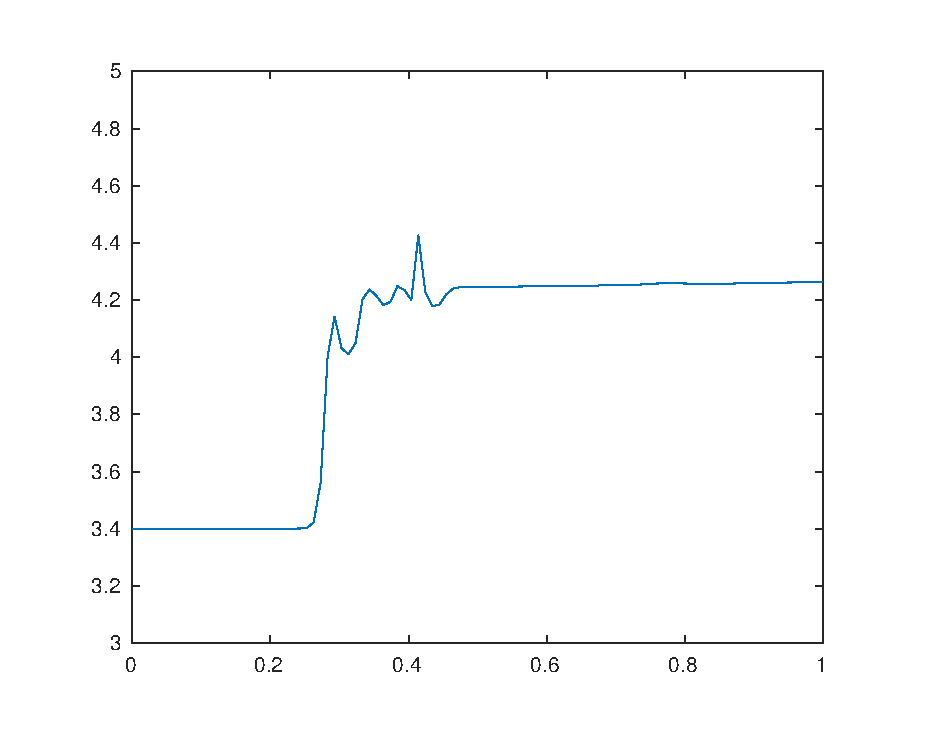
\includegraphics[width=\textwidth]{images/sol_1D_free_0600.eps}
        \caption{$n=600$}
        \label{fig:100}
    \end{subfigure}
     \caption{Free boundary conditions for 1D scheme.}
    \label{fig:1DSolutions_free}
\end{figure}

